% mail pc03_org@nersc.gov <= July 15th with
\documentclass[10pt,fleqn]{article}
\setlength{\mathindent}{0.25in}
\usepackage{graphicx}
\usepackage{latexsym}

\newcommand{\sign}{{\it sign}}
\newcommand{\diag}{{\it diag}}

%*** Column setup
%\setlength{\columnsep}{0.5in}
%\setlength{\columnseprule}{0.01in}

\pagestyle{plain}

%*** Page numbering
%\pagenumbering{arabic}
%\setcounter{page}{1}

%*** Paragraph setup

\setlength{\parindent}{0ex}
\setlength{\parskip}{01.5ex plus 0.3ex minus 0.3ex}
\renewcommand{\baselinestretch}{1.0}

%*** Floats
\renewcommand{\textfraction}{0.01}
\setlength{\floatsep}{0.0in}

%*** Page formating

\setlength{\topmargin}{0.0in}
\setlength{\headheight}{0.3in}
\setlength{\headsep}{0.2in}
\setlength{\textheight}{8.5in}
\setlength{\footskip}{0.5in}

\setlength{\oddsidemargin}{-0.5in}
\setlength{\evensidemargin}{-0.5in}
\setlength{\textwidth}{7in}

%
% Body of document
%
\begin{document}

%
% Title page
%
\title{Preconditioning Techniques in Circuit Simulation}

\author{David M. Day, Michael A. Heroux, Robert J. Hoekstra \\
Sandia National Laboratories\footnote{
Sandia is a multiprogram laboratory operated by Sandia Corporation, a
Lockheed-Martin Company, for the United States Department of Energy
under Contract DE-AC04-94AL85000.}, Albuquerque NM 87185 USA}

\date{\today}

\maketitle

\paragraph{Summary}
This article presents a discussion of
preconditioners for linear systems arising in the 
distributed memory parallel circuit simulation application called
Xyce~\cite{Xyce-home-page}. Xyce is under development at Sandia National Laboratories to
meet Sandia's current and future circuit simulation needs.

The primary computational bottleneck in circuit simulation is the
solution of a sequence of sparse indefinite unsymmetric linear systems
of the form 
\begin{equation}
Ax = b.
\label{Equation1}
\end{equation}
Iterative linear solvers and distributed memory platforms
are needed to meet the demand to simulate circuits with increasing
numbers of devices, a primary goal for Xyce.  

In this article we present a series of approaches to
preconditioning these problems.  We organize the discussion to match
the evolutionary approach we used to develop preconditioners.
Specifically, we first discuss early efforts to solve circuit problems
using well-established methods from PDE applications, and then proceed
to discuss how we specialized these methods for circuits, and explored
new algorithms that address key subproblems in circuit simulation.


\paragraph{Experiments with Standard Preconditioners}
As part of a rapid ramp-up of the first version of Xyce, 
we attempted to use standard overlapping Schwarz preconditioners that are quite effective
for PDE problems.  However, these preconditioners are designed with certain
assumptions about nonzero structure,
overlap, and load balance that reflect their origins.  These assumptions are not appropriate
for circuit problems.

Dense rows and columns, a common feature 
in circuit matrices, made overlapping Schwarz preconditioners
difficult to use.  In these situations, the overlap on one subdomain
can be almost the entire matrix.  Also we observed that incomplete
factorizations often did not exist due to zero diagonals.  Allowing more
fill-in through thresholds was not an efficient solution.  In this stage we 
were forced to rely on the high dimensional Krylov subspaces available
on distributed memory platforms.  

\paragraph{Diagonal Perturbations of ILU and Adaptive Preconditioners}
One technique to improve the effectiveness of standard
incomplete factorizations is to introduce diagonal perturbations.  In
this situation, we compute the factorization of a matrix $B$ that
differs from $A$ in Equation~\ref{Equation1} only on the diagonal.
Specifically, we replace the diagonal values $(d_1, d_2, \ldots, d_n)$
with $d_i = \sign(d_i)\alpha + d_i\rho$, $i=1, 2, \ldots, n$, where
$n$ is the matrix dimension and $\sign(d_i)$ returns
the sign of the diagonal entry.  This has the effect of
forcing the diagonal values to have a minimal magnitude of $\alpha$ and
to increase each value by an amount proportional to $\rho$, and still keep
the sign of the original diagonal entry.

For a matrix $C$, a crude lower bound for the $cond_\infty(C)$ is
$\|C^{-1}e\|_\infty$ where $e = (1, 1, \ldots, 1)^T$.  It is a
lower bound because $cond_\infty(C) = \|C\|_\infty\|C^{-1}\|_\infty
\ge \|C^{-1}\|_\infty \ge |C^{-1}e\|_\infty$.
In our situation, we want to estimate $cond_\infty(LU)$, where $L$ and
$U$ are our incomplete factors.  Chow~\cite{Chow:97} demonstrates that
$\|(LU)^{-1}e\|_\infty$ provides an effective estimate for
$cond_\infty(LU)$.  Furthermore, since finding $z$ such that $LUz = y$
is a basic kernel for applying the preconditioner, computing this
estimate of $cond_\infty(LU)$ is performed by setting $y = e$, calling
the solve kernel to compute $z$ and then
computing $\|z\|_\infty$.

Given the ability to (i) estimate the conditioning of an ILU 
preconditioner and (ii) improve its conditioning 
via diagonal perturbation, we can develop adaptive strategies for
improving robustness of an ILU preconditioned iterative solver.  
The goal when applying {\it a priori} perturbations is to find a close to minimal
perturbation that reduces the condition estimate below machine
precision (roughly 1.0e16). Initially we set the absolute threshold 
$\alpha = 0.0$ and the relative
threshold $\rho = 1.0$ (equivalent to no perturbation) and compute the
incomplete factors $L$ and $U$.  Next we compute 
$condest = \|(LU)^{-1}e\|_\infty$ where $e = (1, 1,
\ldots, 1)^T$. Then,  if $condest > 10^{15}$ or convergence of the
preconditioned iterations is poor,
we alternately increment $\alpha$, and $\rho$ in an attempt improve
the conditioning of the incomplete factorizations and still remain
close enough to the true factorization.  Using this approach in an
automated fashion, greatly improved the robustness of our ILU
preconditioned iterations.

\paragraph{Singleton row and column elimination}

Although adaptive diagonal perturbations greatly improved the robustness of our
incomplete factorizations, we were still unable to reliably use
overlapping domains because many matrices from Xyce contained one or
more rows or columns that were very dense.  This problem has been
effectively addressed by an observation that a dense row
(column) is almost always associated with one column (row) that has a
single entry, and that these row/column pairs can be easily removed from the
original system.  Figure~\ref{singleton_stats} shows the effectiveness
of singleton removal for several Xyce sample problems.  After removal,
these matrix become much closer to matrices that come from PDE
simulations, and the effectiveness of ILU preconditioneing improved substantially.
\begin{figure} 
\begin{center} 
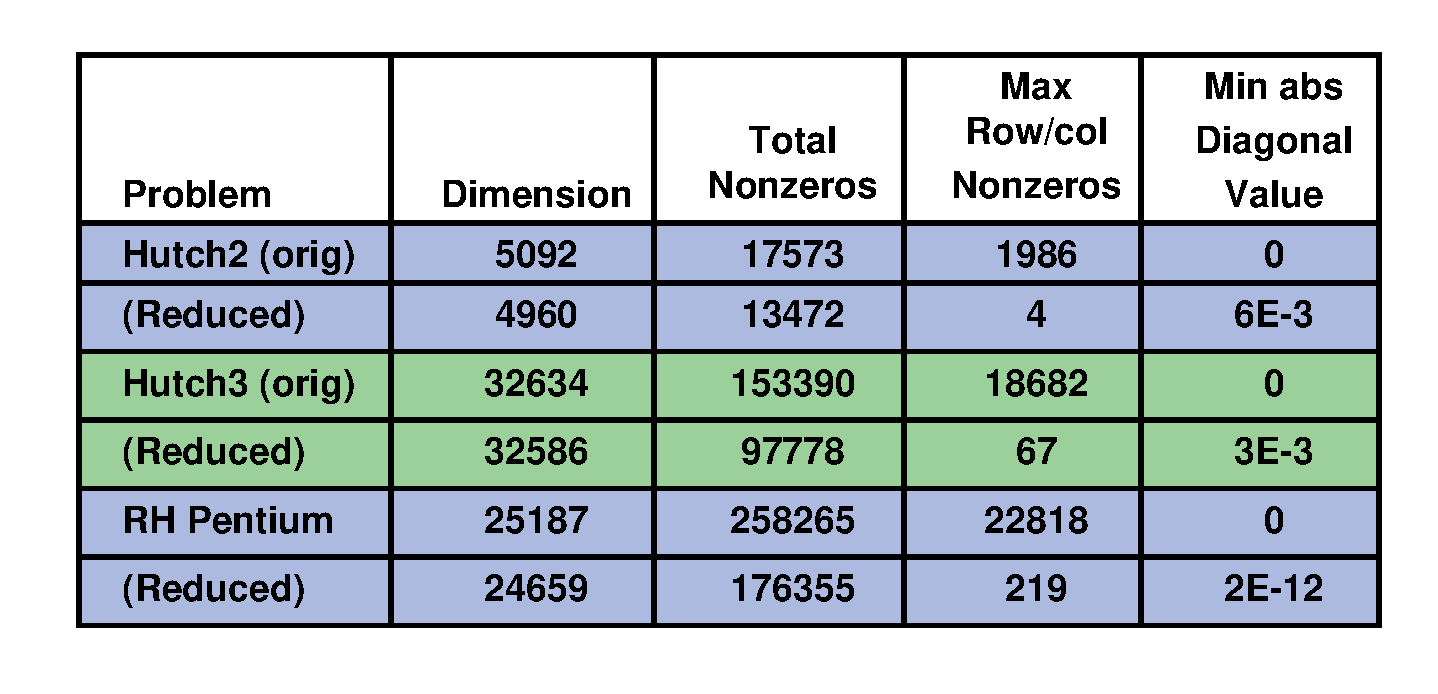
\includegraphics[height=3in]{singleton_stats}
\end{center} 
\caption{\label{singleton_stats} Matrix characteristics before and
after singleton removal.}
\end{figure} 


\paragraph{DC Operating Point Calculations}
Circuit simulation involves nonlinear transient analyses by implicit
differential-algebraic equation solvers using Newton's method.
There is an initial direct current (DC) operating point calculation
that is notoriously difficult, but accounts for
little of the overall computation time.  DC operating point calculations 
involving 1000 Newton iterations are routine and can be a critical
roadblock for particular circuit models.  

We present linear solvers
that exploit the structure of the DC operating point problem.  Specifically,
determining the DC operating point is a steady-state problem that
produces structured Jacobians.  The Jacobians admit a permutation to
block triangular form with small diagonal blocks.  The Dulmage-Mendelsohn
permutation (linear time and memory costs) finds the permutation.

For example, a digital component comprised mainly of MOSFET transistors
is reducible due to the MOSFET's asymmetry.  A MOSFET 'gate' terminal
controls the currents and conductivity for the 'drain', 'source', 
and 'base'.  In steady-state problems through the 'gate' terminal
no current flows and conductivity is zero.  The stencil for the MOSFET
contains a zero row corresponding to the gate.  After permuting the
Jacobian  to lower triangular form, the diagonal blocks are connected
through columns that correspond to the 'gate' terminals.  Transient
problems involve capacitances that generate currents and conductivities
associated with the 'gate', and the Jacobians are irreducible.

The DC operating point Jacobians are often singular.  Analyses using
the singular value decompositions of the diagonal blocks in combination
with condition number estimates for the block triangular system show
that the the diagonal blocks usually support the gravest singular vectors.
Management of rank deficient systems through least squares methods
enhances the convergence of both the linear and the nonlinear solver.

This approach to solving the DC operating point promises to be very 
effective.  Although many nonlinear iterations may still be required,
the linear solve is direct and very efficient since the matrix is
block triangular.  Although we have not done so yet, it is also
possible to isolate coefficients that are associated with
the nonlinearities to further improve the efficiency.

\bibliographystyle{plain}
\nopagebreak
\scriptsize
\bibliography{circuits}
\end{document}

